\subsection{Actualización de elementos}

  \paragraph{}Para editar un elemento del sistema, es necesario pulsar el
  icono \textit{Editar}. Se puede ver una captura de pantalla de este
  icono en la figura \ref{capturaEditElemento}. También es posible acceder
  al formulario de edición del elemento pulsando sobre el nombre del elemento
  que aparece en el listado.

  \begin{figure}[!ht]
    \begin{center}
      \fbox{
      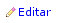
\includegraphics[scale=0.6]{3.Caracteristicas_Interfaz/3.3.Gestion_Informacion/3.3.3.Actualizacion_Elementos/editElemento.png}
      }
      \caption{Captura de pantalla del icono \textit{Editar}.}
      \label{capturaEditElemento}
    \end{center}
  \end{figure}

  \paragraph{}La figura \ref{capturaActualizacionElementos} muestra un ejemplo
  de actualización de un elemento. Como se puede observar, no se diferencia
  de la interfaz de creación de un nuevo elemento, sino que se obtiene la
  información del elemento para su posterior modificación.


  \begin{figure}[!ht]
    \begin{center}
      \fbox{
        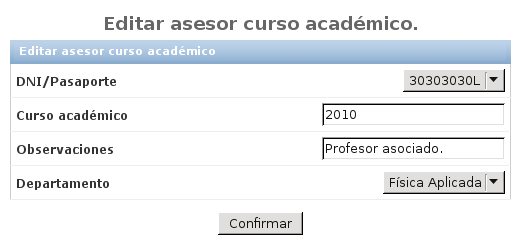
\includegraphics[scale=0.6]{3.Caracteristicas_Interfaz/3.3.Gestion_Informacion/3.3.3.Actualizacion_Elementos/actualizacion_elementos.png}
      }
      \caption{Captura de pantalla de actualización de un elemento.}
      \label{capturaActualizacionElementos}
    \end{center}
  \end{figure}